\documentclass[12pt,a4paper]{article}
\usepackage{amssymb}

\usepackage[spanish,es-tabla]{babel}
\usepackage[a4paper,bindingoffset=0.1in,%
left=0.75in,right=0.75in,top=1in,bottom=1in,%
footskip=.2in]{geometry}
\usepackage[utf8]{inputenc} % Escribir con acentos, ~n...
\usepackage{eurosym} % s´ımbolo del euro
\newcommand{\horrule}[1]{\rule{\linewidth}{#1}} % Create horizontal rule command with 1 argument of height
\usepackage{listings}             % Incluye el paquete listing
\usepackage[cache=false]{minted}
\usepackage{graphics,graphicx, float} %para incluir imágenes y colocarlas
\usepackage{hyperref}
\hypersetup{
	colorlinks,
	citecolor=black,
	filecolor=black,
	linkcolor=black,
	urlcolor=black
}
\usepackage{multirow}
\usepackage{array}
\usepackage{diagbox}
\usepackage{amsmath}
\usepackage{verbatim}
\begin{document}

\title{Aprendizaje autom\'atico. Cuestionario 3}

\author{
  Antonio Jesús Heredia Castillo\\
  \texttt{xxxxxxxx}
}

\date{}
\maketitle
\horrule{2pt}

\begin{enumerate}
	\item ¿Podría considerarse Bagging como una técnica para estimar el error de predicción de un
modelo de aprendizaje?. Diga si o no con argumentos. En caso afirmativo compárela con
	validación cruzada.\\\\
	\textbf{Respuesta: }\\
	Si, ya que usa para generar los conjuntos de entrenamiento bootstraping. Se puede medir el error usando la tecnica OOB (out-of-bag).\\
	Una diferencia es que en validación cruzada  hacemos una división de los datos y trabajamos con cada parte por separado, no se repiten datos. En cambio Bagging como he dicho antes, usa bootstraping para  generar nuevas muestras y esto lo realiza remuestreando de forma aleatoria y con remplazo. Por lo tanto se pueden repetir datos en los diferentes conjuntos.
	
	 
	\item Considere que dispone de un conjunto de datos linealmente separable. Recuerde que una
vez establecido un orden sobre los datos, el algoritmo perceptron encuentra un hiperplano
separador interando sobre los datos y adaptando los pesos de acuerdo al algoritmo.
\begin{figure}[H]
	\centering
	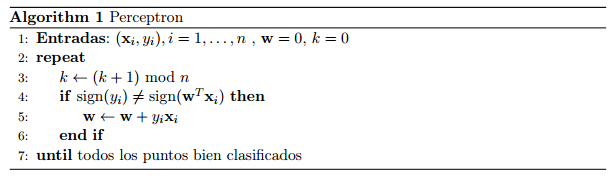
\includegraphics[width=0.7\linewidth]{perceptron}

	\label{fig:perceptron}
\end{figure}

	Modificar este pseudo-código para adaptarlo a un algoritmo simple de SVM, considerando
	que en cada iteración adaptamos los pesos de acuerdo al caso peor clasificado de toda la
	muestra. Justificar adecuadamente/matematicamente el resultado, mostrando que al final
	del entrenamiento solo estaremos adaptando los vectores soporte.

	\item Considerar un modelo SVM y los siguientes datos de entrenamiento: $Clase-1:{(1,1),(2,2),(2,0)}$, $Clase-2:{(0,0),(1,0),(0,1)}$

	\begin{enumerate}
		\item Dibujar los puntos y construir por inspección el vector de pesos para el hiperplano óptimo y el margen óptimo.
		\\	\textbf{Respuesta: }\\
		La separación optima seria la recta que pasa por los puntos $(0.5,1)$ y $(1.5,0)$. Ya que dejaria un margen de $\sqrt{0.5}=0.7071$
		\begin{figure}[H]
			\centering
			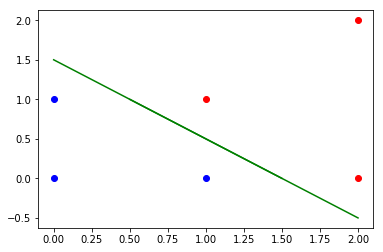
\includegraphics[width=0.7\linewidth]{porInspeccion}
	
			\label{fig:porinspeccion}
		\end{figure}
		\item ¿Cuáles son los vectores soporte?
		\\	\textbf{Respuesta: }\\
		Por un lado tendriamos el $\{(0,1)(1,0)\}$ y por otro el $\{(1,1)(2,0)\}$. Los vectores serian las lineas moradas. 
		\begin{figure}[H]
			\centering
			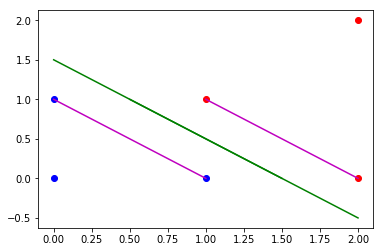
\includegraphics[width=0.7\linewidth]{vectoresSoporte}

			\label{fig:vectoressoporte}
		\end{figure}
		
		\item Construir la solución en el espacio dual. Comparar la solución con la del apartado (a)		\\	\textbf{Respuesta: }\\
\begin{figure}[H]
	\centering
	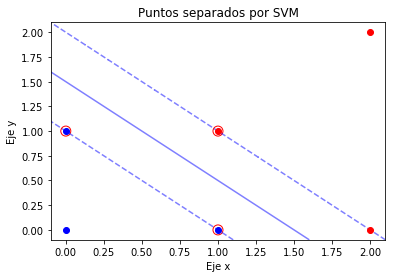
\includegraphics[width=0.7\linewidth]{screenshot001}

	\label{fig:screenshot001}
\end{figure}
Usando un ``C'' (penalización), lo suficientemente grande tendremos una solución igual que la optima. 



	\end{enumerate}
		\item ¿Cual es el criterio de optimalidad en la construcción de un árbol? Analice un clasificador
		en árbol en términos de sesgo y varianza. ¿Que estrategia de mejora propondría? 
		\\\\	\textbf{Respuesta: }\\
		\item ¿Cómo influye la dimensión del vector de entrada en los modelos: SVM, RF, Boosting and
NN?.
		\\\\	\textbf{Respuesta: }\\
		En 	\textbf{SVM} no importa  si tenemos una gran dimensión el vector de características. Ya que es capaz de generalizar y regularizar para evitar efectos adversos. 
		\\
		En 	\textbf{random forest} al construir arboles no correlados tampoco influye que los vectores de caracteristicas sean muy grandes. 
		\\
		En 	\textbf{NN} vamos a necesitar normalmente un numero exponencial de capas ocultas en relación con la dimension del vector de caracteristicas, por lo tanto cuanto mayor sea, mas capas necesitaremos.
		\\
		En \textbf{boosting} aunque se puede evitar el sobre ajuste para dimensiones grandes maximizando el margen, esto tendrá un coste computación muy grande.
		
		\item El método de Boosting representa una forma alternativa en la búsqueda del mejor clasificador
respecto del enfoque tradicional implementado por los algoritmos PLA, SVM, NN, etc. a) Identifique de forma clara y concisa las novedades del enfoque; b) Diga las razones profundas
por las que la técnica funciona produciendo buenos ajustes (no ponga el algoritmo); c) Identifique sus principales debilidades; d) ¿Cuál es su capacidad de generalización comparado
		con SVM?
		
		\item Discuta pros y contras de los clasificadores SVM y Random Forest (RF). Considera que
		SVM por su construcción a través de un problema de optimización debería ser un mejor
		clasificador que RF. Justificar las respuestas.\\
		 
		\textbf{SVM}
		\\Pros: Funciona muy bien cuando la dimensión es muy alta. No necesita todos los datos, con los vectores soporte ya consigue el hiperplano que separa a estos. Si no hay ruido consigue un optimo global. 
		\\Contras: Puede tener overfitting. Dificultad a la hora de elegir un buen Kernel para el problema. Solo se pueden separar los datos sin son linealmente separables.
		\\
		\textbf{Random Forest}
		\\
		 
		\item ¿Cuál es a su criterio lo que permite a clasificadores como Random Forest basados en
		un conjunto de clasificadores simples aprender de forma más eficiente? ¿Cuales son las
		mejoras que introduce frente a los clasificadores simples? ¿Es Random Forest óptimo en
		algún sentido? Justifique con precisión las contestaciones. \\\\
		\textbf{Respuesta}\\
		Como crea varios modelos simples a partir de datos cogidos de forma aleatoria y combinamos  estos modelos, obtenemos una baja varianza y tener al modelo entrenado para distintas situaciones.\\
		La mejora que introduce es que al usar Baggin baja la varianza. \\
		Si, ya que trabaja facilmente con dataset grandes, teniendo suficientes datos genera un clasificador muy certero y no excluye variables de entrada.
		
		\item En un experimento para determinar la distribución del tamaño de los peces en un lago, se
		decide echar una red para capturar una muestra representativa. Así se hace y se obtiene
		una muestra suficientemente grande de la que se pueden obtener conclusiones estadísticas
		sobre los peces del lago. Se obtiene la distribución de peces por tamaño y se entregan las
		conclusiones. Discuta si las conclusiones obtenidas servirán para el objetivo que se persigue
		e identifique si hay algo que lo impida.
		\\\\		\textbf{Respuesta: }\\
		Al echar la red de forma aleatoria  no podemos asegurar que obtengamos una muestra suficientemente representativa. Ni en el enunciado nos dicen la distribución de la muestra.\\ Podemos haber lanzado la red en una zona donde solo se encuentra un determinado de pez pero en la otra parte del rio haya otro tipo de pez. \\ 
		Desde mi punto de vista hubiera sido mejor echar la red en varios sitios cogiendo menos peces de cada vez, pero de esta forma posiblemente hubiera sido mas representativa. 
		
		\item  Identifique que pasos daría y en que orden para conseguir con el menor esfuerzo posible un
		buen modelo de red neuronal a partir una muestra de datos. Justifique los pasos propuestos,
		el orden de los mismos y argumente que son adecuados para conseguir un buen óptimo.
		Considere que tiene suficientes datos tanto para el ajuste como para el test.
		\\\\		\textbf{Respuesta: }\\
		Los primeros pasos serian recolectar los datos, ya que tener una muestra de datos lo suficientemente representativa es esencial para que el resultado del modelo sea bueno.\\
		El segundo paso es el preprocesamiento de los datos. Tenemos que ver que caracteristicas son importantes, hacer normalización en caso de que sea necesario y realizar regularización de los datos. Tambien seria necesario en este paso separar los datos para entrenamiento y test y en caso de que se vaya a realizar validación otro conjunto para ese caso.\\
		Como ya sabemos que el modelo que vamos a usar es redes neuronales, en este punto deberiamos elegir 3 cosas importantes. Cuantas capas va a tener nuestra red, cuantas neuronas por capas y cual sera la función de activación. 
		\\
		Ahora debemos ver valor para los hiperparametros vamos a usar e ir haciendo ``tuning'' hasta que tengamos un modelo entrenado de forma convincente. 
\end{enumerate}
\clearpage

\end{document}
